\chapter{Web-Visualisierung}\thispagestyle{fancy}

\section{Arbeitsverteilung/ Zielstellung}

\Large
{Ab November soll ein neues Projekt entstehen, welches das Ziel hat, einige gemessene und gesendete Daten einer Kraftwerk, mittels eine Website  visualisieren. Am Anfang war das Projekt-Zielstellung besprochen worden. In diese Besprechungen wurden die jeweiligen Aufgaben verteilt. Die Abteilung Eingebete Systeme soll einen Apache Server mit PHP installieren und eine postgreSQL Datenbank, wo alle Werten aus eine Kraftwerk gespeichert werden, erstellen. Mir war die Visualisierung von diese Daten zugeordnet. Die visualisierte Daten sollen in einer Website dargestellt werden. \\
Die Daten aus einer Kraftwerk sollen �bersichtlich und mittels Diagrammen visualisiert werden. Es war festgelegt, welche Daten zu visualisieren geeignet sind. Es war auch besprochen, welche Mitteln f�r die Website Erstellung geeignet sind. Dazu geh�ren Bootstrap Frameworks, jQuery und dazugeh�rige Software f�r die Bearbeitung.}

% erstmals einen Projekt Plan erstellt, Besprechung\\

% jeweiligen aufgaben verteilen = Eingebete Systeme sollen eine Apache Server mit PHP, ich soll die Website, Design und Konzept entwickeln\\

% definieren was wird visualisiert, Was ist unsere ziel? (genauer definieren) = Daten eine Kraftwerk �bersichtlich darstellen und im Diagrammen anzeigen\\


\section{Konzipierung}

\Large{Es soll ein Konzept f�r die Website entwickelt werden. Es wird ein Konzept mit grafisches Programm GIMP gemacht, wo ich erste Konzepte f�r die Anmeldung-Seite (siehe Abbildung \ref{login_seite}) und f�r die Seite, wo die jeweiligen L�nder und Anlagen angezeigt werden (siehe Abbildung \ref{Anlagenblocke}), gemacht habe. Es war auch gebraucht einen Konzept f�r die Seite mit eine Auswahl von L�nder zu entwickeln. Da ist meine Abteilung auf der Idee gekommen, dass wir eine gro�e Karte mit Zeigers/Pointers in die Seite implementieren werden, wo der Benutzer aus der jeweiligen Region/Land ein Kraftwerk ausw�hlen kann. Es wurden auch erste Konzepte f�r die Tabellen, Fehlermeldungen und Diagrammen gemacht.}

% Mittels grafischer Soft und Papier habe ich zu erst Konzepte f�r die Website erstellt, Ideen wie es aussehen soll, dann wieder besprechen

% Interface, wie soll die Seite aussehen = Tabellen, Reports, Fehlern, Diagramme, Men�-Auswahl Liste mit Modulen, Auswahl von L�ndern, Kraftwerken

\vspace{0,5cm}

\begin{figure}[htbp]
	\centering
		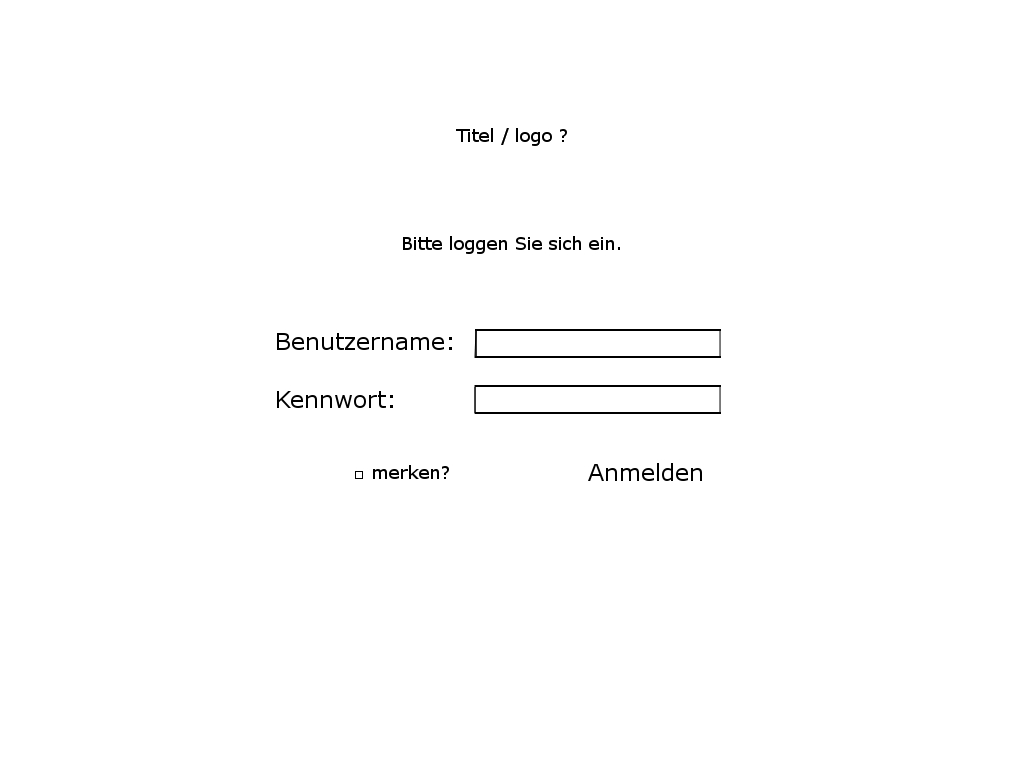
\includegraphics[width=0.7\textwidth]{images/start_login.jpg}
		\caption{Login-Seite}
		\label{login_seite}
\end{figure}

\vspace{0,5cm}

\begin{figure}[htbp]
  \centering
     \subfigure[Vor dem Klick]{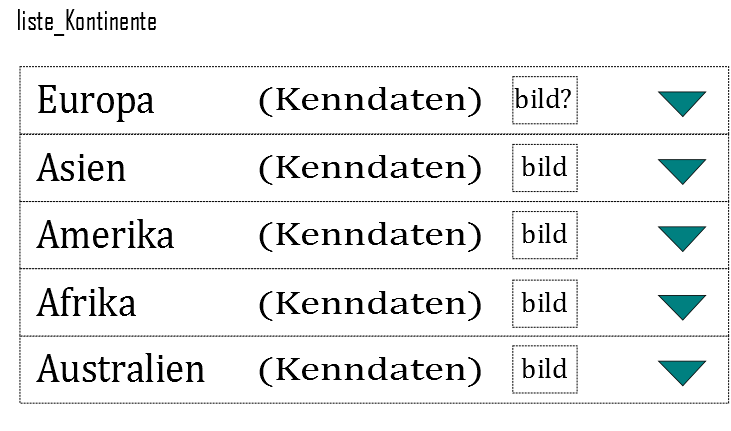
\includegraphics[width=0.4\textwidth]{images/Liste_Kontinente.PNG}}
			\hspace{1cm}
		 \subfigure[Nach dem Klick]{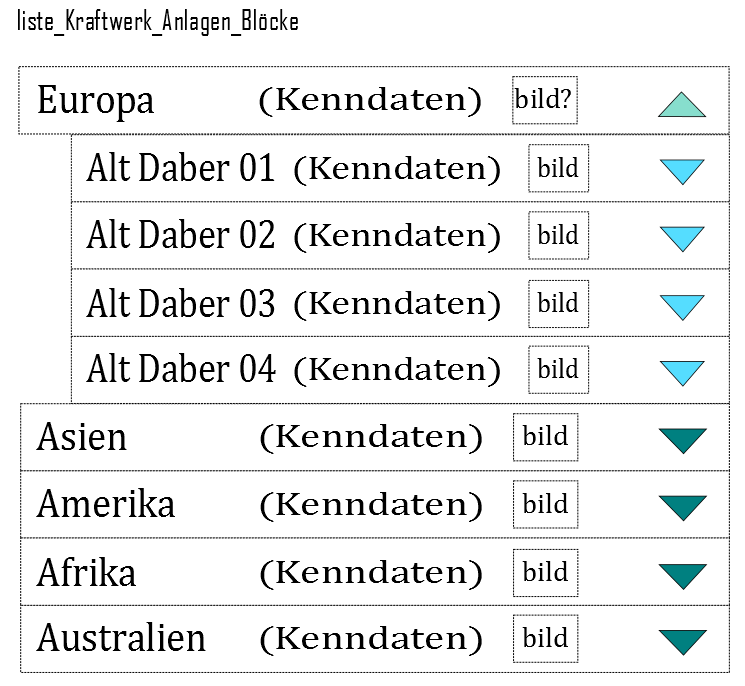
\includegraphics[width=0.4\textwidth]{images/Liste_Anlagenblocke.PNG}}
	\caption{Liste mit L�nder und Anlagen}
  \label{Anlagenblocke}
\end{figure}

\section{Website - Entwicklung}

\Large{N�chste Aufgabe war, die entwickelte Konzepte in statisches HTML mit CSS und Javascript umzusetzen. Unser Team hat abgesprochen, dass wir f�r die Website Entwicklung das Bootstrap Frameworks benutzen werden. Das hat sehr viele Vorteile, als beim Null zu starten. Erstens ist das Bootstrap auch f�r kommerzielle Benutzung kostenlos, zweitens es beschleunigt die Arbeit, weil es sozusagen schon die CSS-Programmierung gemacht hat und wir nutzen nur die vorkonfiguriertes CSS Style f�r die jeweiligen HTML Elementen und drittens Bootstrap bietet sehr kompatible und responsive Design, das hei�t, dass die Seite auch f�r alle Browsers sowie Handys und Tabletts optimiert ist. F�r Programmieren habe ich das Software Sublime Text benutzt.\\
Das erste Konzept der Login-Seite war mit Bootstrap gemacht (siehe Abbildung \ref{login_seite_boot}), eine einfache HTML Seite mit Belectric Logo, Anmeldungsfelder und einen Button 'Sign In'.\\}


\begin{figure}[htbp]
	\centering
		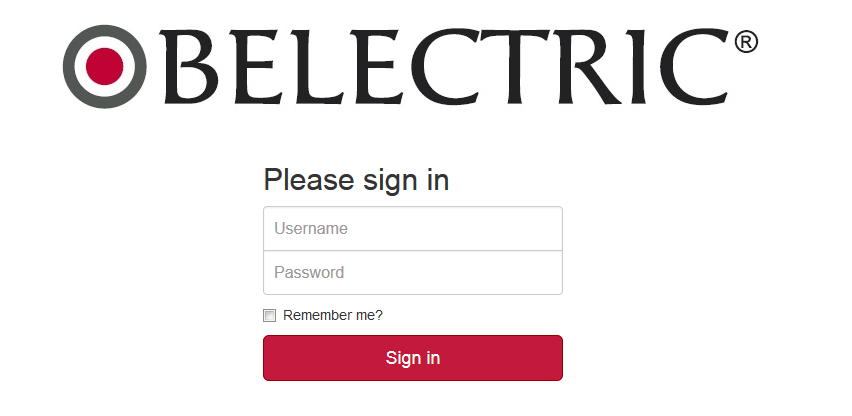
\includegraphics[width=0.8\textwidth]{images/login_seite_boot.png}
		\caption{Login-Seite mit Bootstrap}
		\label{login_seite_boot}
\end{figure}


\Large{Es wird danach der Konzept der Auswahl-Liste mittels HTML und Bootstrap realisiert. Mit dem Bootstrap kann man schnell die Liste erstellen und auch die Breite jedes Listenelement mit HTML \textbf{class}-en einstellen. Daf�r dient sogenannte Grid System, welchen Bootstrap entwickelt hat. Es funktioniert so, dass die Breite einen erstellten \textbf{div} mit \textbf{collums} mit unterschiedliche Gro�e einstellbar ist. Mit der maximale Breite 13 wird es so geschrieben: \textbf{col-lg-13} bzw. \textbf{col-sm-13}. Das, was in diesem \textbf{div} dargestellt wird, wird sich auch �ber die ganze Breite der Seite strecken.\\
In unseren Fall, war \textbf{col-lg-8} f�r die Kontinente eingestellt und einen \textbf{col-lg-offset-1} f�r die untergeordnete Liste mit L�nder, damit die um einen col-1 verschoben wird.\\}

\begin{figure}[htbp]
	\centering
		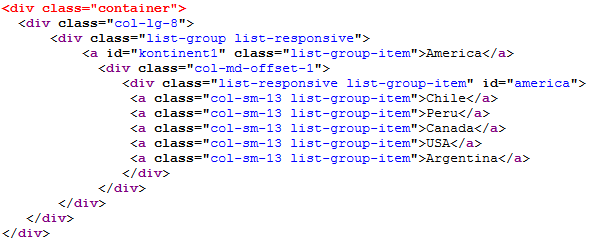
\includegraphics[width=1\textwidth]{images/html_list_kontinente.png}
		\caption{Liste mit Amerika}
		\label{html_list_kontinente}
\end{figure}

\section{Website online machen}

\Large{Kollegen haben einen Server erstellt, wo ich die Website ver�ffentlichen soll, damit die online verf�gbar ist}

\section{Die postgreSQL-Datenbank}

\Large{Verbinden von Daten aus SQL, Meta-Datenbank erstellt, welche die Allgemeine Infos und Daten zu Kraftwerk beinhaltet, Einen System erstellt und die Datenbank �ber SQL Sprache erstellt}



\section{Dynamische Umsetzung (PHP)}

\Large{Eine Dynamische Umsetzung erfolgt mittels PHP und andere.. es ist wichtig, dass die Seite dynamisch funktioniert, dass es automatisiert ist und wenn wir die SQL erweitern dann wird es automatisch im Website angezeigt}

% Key-Features: die Ajax Abfragen - aktualisieren von Daten, Daten aus der EBU, WR, BMS, Pool und evtl. noch weiteren visualisieren\\



\section{Daten Visualisieren}

\Large{Die Daten die im SQL liegen werden mittels Diagrammen visualisiert, es gibt mehrere Diagrammen-Bibliotheken, die man benutzen kann,  es war wichtig, dass die Open-source, mit SQL arbeiten kann - dynamisch, viele Optionen wie Export, mehrere Linien anzeigen, mehrere Typen von Charts, Datum-anzeigen}

% Charts-Plattform, welche Diagramm-Bibliothek benutzen wir? = meine Aufgabe war eine Auswahl von Charts machen, den besten finden und lernen damit die Daten visualisieren\\